  \let\negmedspace\undefined
\let\negthickspace\undefined
\documentclass[journal]{IEEEtran}
\usepackage[a5paper, margin=10mm, onecolumn]{geometry}
\usepackage{lmodern} % Ensure lmodern is loaded for pdflatex
\usepackage{tfrupee} % Include tfrupee package

\setlength{\headheight}{1cm} % Set the height of the header box
\setlength{\headsep}{0mm}     % Set the distance between the header box and the top of the text

\usepackage{gvv-book}
\usepackage{gvv}
\usepackage{cite}
\usepackage{amsmath,amssymb,amsfonts,amsthm}
\usepackage{algorithmic}
\usepackage{graphicx}
\usepackage{textcomp}
\usepackage{xcolor}
\usepackage{txfonts}
\usepackage{listings}
\usepackage{enumitem}
\usepackage{mathtools}
\usepackage{gensymb}
\usepackage{comment}
\usepackage[breaklinks=true]{hyperref}
\usepackage{tkz-euclide} 
\usepackage{listings}                                      
\def\inputGnumericTable{}                                 
\usepackage[latin1]{inputenc}                                
\usepackage{color}                                            
\usepackage{array}                                            
\usepackage{longtable}
\usepackage{multicol}
\usepackage{calc}                                             
\usepackage{multirow}                                         
\usepackage{hhline}                                           
\usepackage{ifthen}                                           
\usepackage{lscape}
\begin{document}

\bibliographystyle{IEEEtran}
\vspace{3cm}

\title{9.3.11}
\author{EE24BTECH11024 - G. Abhimanyu Koushik}
% \maketitle
% \newpage
% \bigskip
{\let\newpage\relax\maketitle}

\renewcommand{\thefigure}{\theenumi}
\renewcommand{\thetable}{\theenumi}
\setlength{\intextsep}{10pt} % Space between text and floats


\numberwithin{equation}{enumi}
\numberwithin{figure}{enumi}
\renewcommand{\thetable}{\theenumi}


\textbf{Question}:\newline
Solve the differential equation $\frac{d^2y}{dx^2} = y$ with initial conditions $y\brak{0} = 1$ and $y^{\prime}\brak{0} = 0$
\newline
\textbf{Solution: }
\newline
Theoritical Solution:\\
Laplace Transform definition\\
\begin{align}
	\mathcal{L}\brak{f\brak{t}} = \int_{0}^{\infty}e^{-st}f\brak{t}dt
\end{align}
Properties of Laplace tranform
\begin{align}
	\mathcal{L}\brak{y^{\prime\prime}} &= s^2\mathcal{L}\brak{y} -sy\brak{0}-y^\prime\brak{0}\\
	\mathcal{L}\brak{1} &= \frac{1}{s}\\
	\mathcal{L}\brak{cf\brak{t}} &= c\mathcal{L}\brak{f\brak{t}}\\
	\mathcal{L}\brak{f\brak{t}} = F\brak{s} &\implies \mathcal{L}\brak{e^{at}f\brak{t}} = F\brak{s-a}
\end{align}
Applying the properties to the given equation
\begin{align}
	y^{\prime\prime} - y &= 0\\
	\mathcal{L}\brak{y^{\prime\prime}} - \mathcal{L}\brak{y} &= 0\\
	s^2\mathcal{L}\brak{y} -sy\brak{0}-y^\prime\brak{0}-\mathcal{L}\brak{y} &= 0\\
\end{align}
Substituting the initial conditions gives
\begin{align}
	\brak{s^2-1}\mathcal{L}\brak{y}&= s\\
	\mathcal{L}\brak{y} &= \frac{s}{s^2 - 1}\\
	 \mathcal{L}\brak{y} &= \frac{1}{2\brak{s+1}}+\frac{1}{2\brak{s-1}}\\
	y &= \frac{1}{2}\brak{\mathcal{L}^{-1}\brak{\frac{1}{s+1}}+\mathcal{L}^{-1}\brak{\frac{1}{s-1}}}\\
	y &= \frac{1}{2}\brak{e^{-x}+e^{x}}u\brak{x}
\end{align}
The theoritical solution is 
\begin{align}
	f\brak{x} = \frac{1}{2}\brak{e^{-x}+e^{x}}u\brak{x}
\end{align}
\newline
Computational Solution:\newline
The given differential equation is
\begin{align}
	y^{\prime\prime} - y = 0
\end{align}
Let
\begin{align}
	y^\prime = y_1\\
	y = y_2
\end{align}
Then
\begin{align}
	\frac{dy_1}{dx} &= y_2\\
	\frac{dy_2}{dc} &= y_1\\
	\int_{y_{1,k}}^{y_{1,k+1}}dy_1 &= \int_{x_k}^{x_{k+1}}y_2dx\\
	\int_{y_{2,k}}^{y_{2,k+1}}dy_2 &= \int_{x_k}^{x_{k+1}}y_1dx
\end{align}
Discretizing the steps using trapezoidal rule gives us
\begin{align}
	y_{1,k+1} - y_{1,k} = \frac{h}{2}\brak{y_{2,k}+y_{2,k+1}}\\
	y_{2,k+1} - y_{2,k} = \frac{h}{2}\brak{y_{1,k}+y_{1,k+1}}
\end{align}
Then solving for $y_{1,k+1}$ and $y_{2,k+1}$ in terms of $y_{1,k}$, $y_{2,k}$ and $h$ will help us to calculate the value of function at $x_{k+1}$
\begin{align}
	y_{1,k+1} = y_{1,k} + \frac{h}{2}\brak{y_{2,k}+\brak{y_{2,k}+\frac{h}{2}\brak{y_{1,k}+y_{1,k+1}}}}\\
	y_{1,k+1} = y_{1,k}\brak{1+\frac{h^2}{4}} + y_{2,k}h + y_{1,k+1}\brak{\frac{h^2}{4}}\\
	y_{1,k+1}\brak{1-\frac{h^2}{4}} = y_{1,k}\brak{1+\frac{h^2}{4}} + y_{2,k}h\\
	y_{1,k+1} = \frac{\brak{y_{1,k}}\brak{4+h^2}+4h\brak{y_{2,k}}}{4-h^2}
\end{align}
Similarly
\begin{align}
y_{2,k+1} = \frac{\brak{y_{2,k}}\brak{4+h^2}+4h\brak{y_{1,k}}}{4-h^2}
\end{align}
The difference equations are
\begin{align}
y_{1,k+1} = \frac{\brak{y_{1,k}}\brak{4+h^2}+4h\brak{y_{2,k}}}{4-h^2}\\
y_{2,k+1} = \frac{\brak{y_{2,k}}\brak{4+h^2}+4h\brak{y_{1,k}}}{4-h^2}
\end{align}
Using the above formula, recording the value of $y$ at each value of $x_{k} = x_0 + kh$ and taking $y\brak{0} = 1$ and $y^\prime\brak{0}=0$ and plotting gives
\begin{figure}[h!]
   \centering
   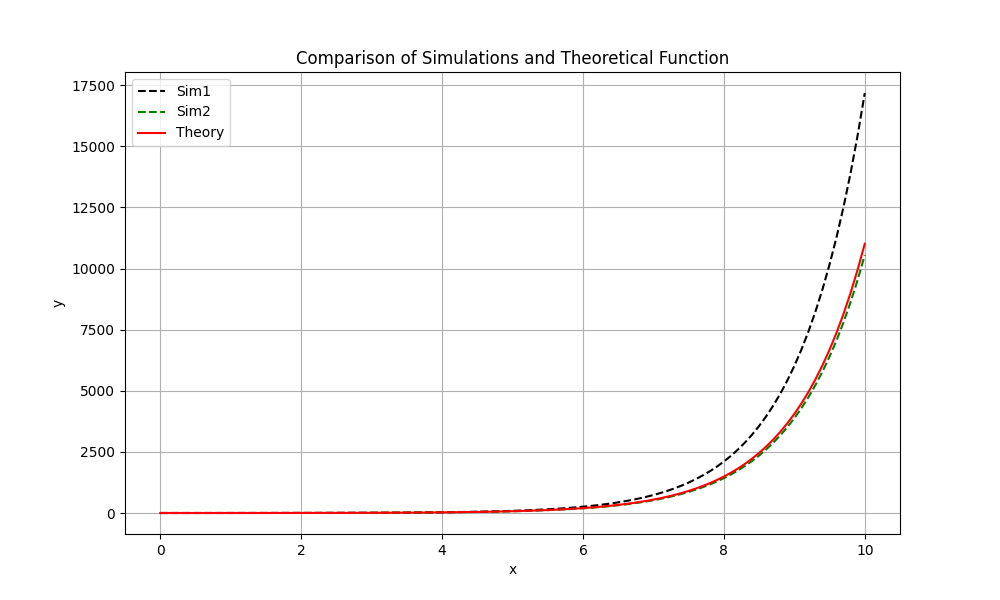
\includegraphics[width=\columnwidth]{figs/fig.png}
   \caption{Comparison between the Theoritical solution and Computational solution}
   \label{stemplot}
\end{figure}
\end{document}  
